\section{Randomness}

	Until now, every transformation had a deterministic figure.
	Usually, for fractals, this is a important behavior but sometimes some randomness would be useful.
	For example suppose we want to simulate some trees.
	Every tree created should have a different type of transformation.
	Even if we use different starting segments, the trees will have similar behavior.
	What to do then in order to create a forest of trees.
	Randomness is the answer.

	In his book ``A new Kind of Science'', Stephen Wolfram discusses about the fact that randomness can arise from within a simple system without interaction from other systems (external factors).
	For exemplifying this, he uses different types of finite automata.

	In finite automata, the further development of a cell can be influenced by it's surroundings.
	His finite automata are placed in discrete space and can easily have access to their surroundings.
	I found it harder to reproduce this behavior for systems which are placed in continuous space.

	For example a segment could recurse further or stop depending on whether it crosses another segment.
	Or the type of the segment could be influenced by the number of segments in a certain proximity.

	The implementation of these functionalities into the software would take away its minimalism.
	That is the reason I chose (for now) some other methods for creating randomness.
	Unfortunately these methods rely on external factors.

	\subsection{Node position variation}

		Suppose we have setup of a simple tree (fig.~\ref{ran_tree_01}).
		It will create a very basic fractal.
		In order to add some randomness the following should be done by the user.
		Press \emph{CTRL} key while dragging the node.
		A blue disc appears around the node (fig.~\ref{ran_tree_02}).
		This blue disc represents the area in which the node can be placed.
		To delete the randomness disc press the \emph{CTRL} key and the middle mouse button.

		One can observe that the creating, deletion buttons retain their meaning,
			only the \emph{CTRL} key is added.

		\begin{figure}[H]
			\centering
			\subcaptionbox{\label{ran_tree_01} A simple tree.}[0.4\textwidth]
				{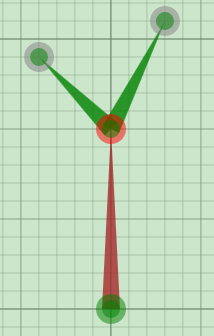
\includegraphics[height=0.3\textwidth]{img/Randomness/Node/ran_tree_01.png}}
			~
			\subcaptionbox{\label{ran_tree_02} A tree with added randomness.}[0.4\textwidth]
				{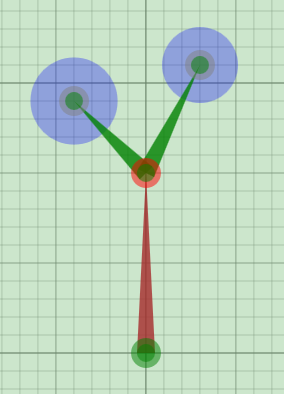
\includegraphics[height=0.3\textwidth]{img/Randomness/Node/ran_tree_02.png}}
		\end{figure}

		Figure~\ref{ran_tree_03} shows some possible trees.
		All the trees were created using the same starting segment.

		\begin{figure}[H]
			\centering
			\caption{\label{ran_tree_03} Some random trees.}
			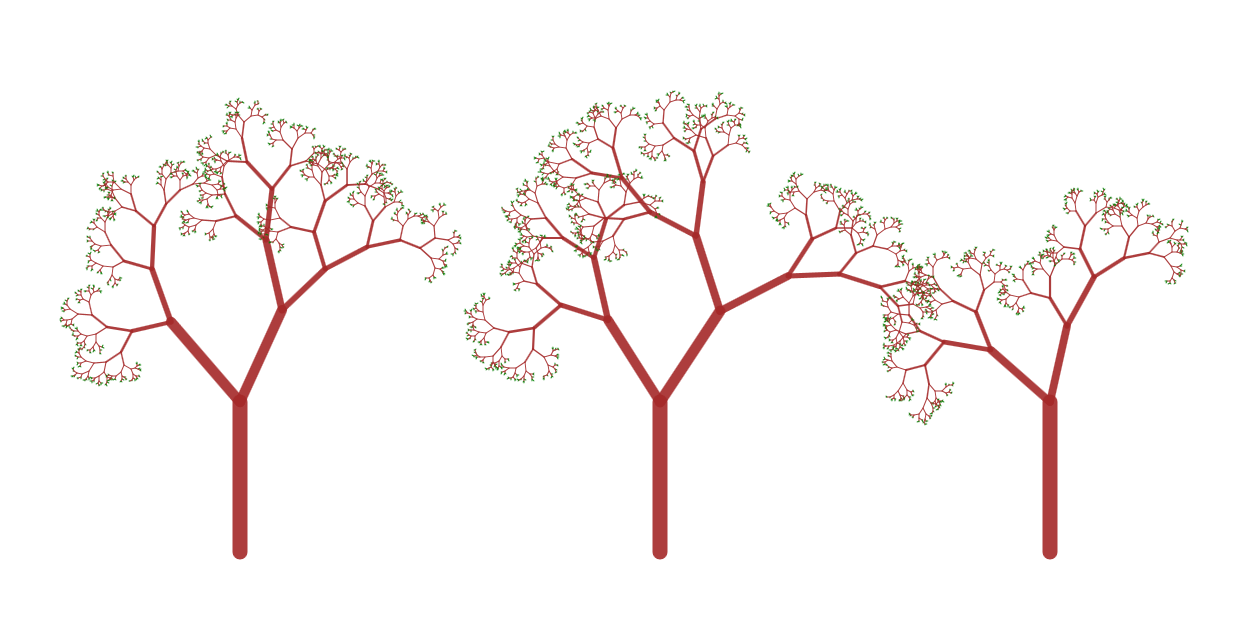
\includegraphics[width=0.9\TW]{img/Randomness/Node/ran_tree_03.png}
		\end{figure}

		The start point and the end point cannot have a random position.
		No node in the base layer can have a random position.

		Let's look at some useful application.

		\subsubsection{Random Paths}

			The setup of a very interesting example can be observed in figure~\ref{ran_path_set_01}.
			Figure~\ref{ran_path_01} shows some of the figures, superimposed.

			\begin{figure}[H]
				\centering
				\caption{Random path.}
				\subcaptionbox{\label{ran_path_set_01} The setup.}[0.3\textwidth]
					{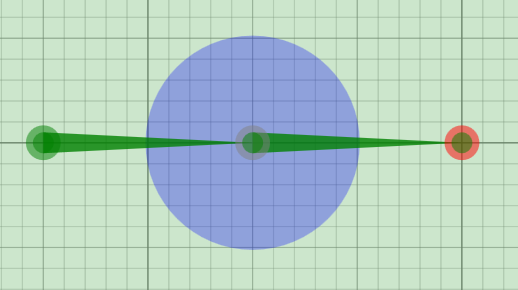
\includegraphics[width=0.29\TW]{img/Randomness/Node/ran_path_01.png}}
				~
				\subcaptionbox{\label{ran_path_01} Some paths.}[0.6\textwidth]
					{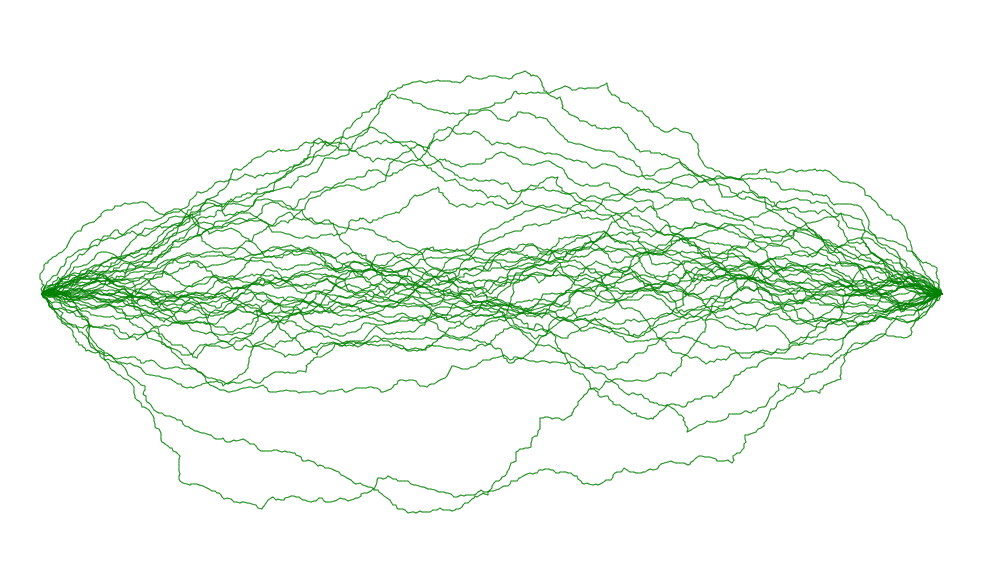
\includegraphics[width=0.59\TW]{img/Randomness/Node/ran_path_02.png}}
			\end{figure}

		\subsubsection{Random Spirals}

			Due to the minimalistic nature of spirals, randomness is a very good fit for them.
			I'll start with spirals which do not rotate.

			\begin{figure}[H]
				\centering
				\caption{Straight spirals.}
				\subcaptionbox{\label{ran_spir_set_01} The setup.}[0.3\textwidth]
					{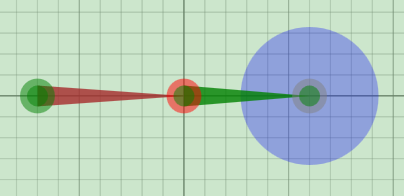
\includegraphics[width=0.29\TW]{img/Randomness/Node/ran_spir_set_01.png}}
				~
				\subcaptionbox{\label{ran_spir_01} Some paths.}[0.6\textwidth]
					{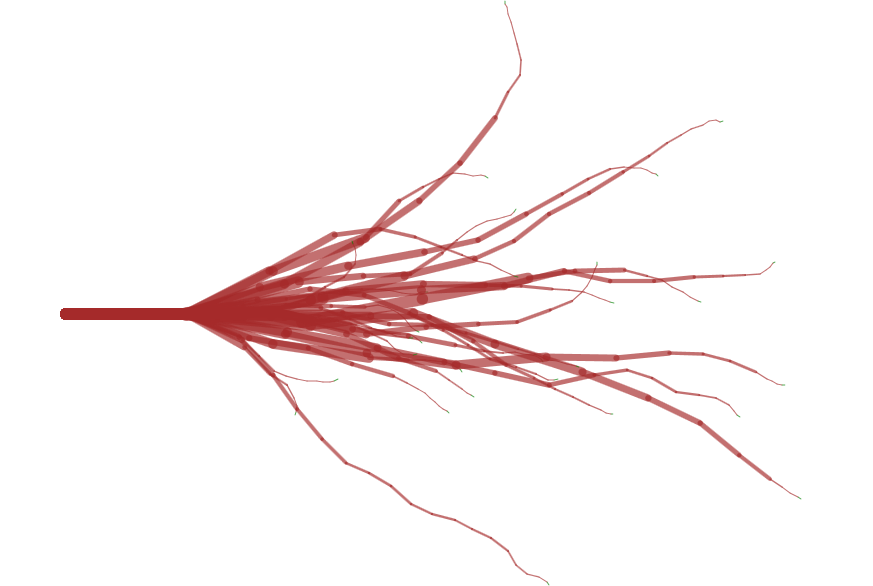
\includegraphics[width=0.59\TW]{img/Randomness/Node/ran_spir_01.png}}
			\end{figure}

			Randomness can be applied to \quotes{real} spirals but that doesn't always result in a beautiful picture.

			\begin{figure}[H]
				\centering
				\caption{\label{ran_spir_02} Some spirals.}
				
\includegraphics[width=0.29\TW]{img/Randomness/Node/ran_spir_02.png}
				
\includegraphics[width=0.29\TW]{img/Randomness/Node/ran_spir_03.png}
				
\includegraphics[width=0.29\TW]{img/Randomness/Node/ran_spir_04.png}
			\end{figure}